%
% einleitung.tex -- Beispiel-File für die Einleitung
%
% (c) 2020 Prof Dr Andreas Müller, Hochschule Rapperswil
%
% !TEX root = ../../buch.tex
% !TEX encoding = UTF-8
%
\section{Ein moderner Beweis
\label{basel:section:moderner-beweis}}
\kopfrechts{Ein moderner Beweis}

Betrachtet wird die Funktion $x \mapsto x^2$ auf $[-\pi, \pi)$.
Zur Analyse dieser Funktion eignet sich die Fourier-Analyse besonders gut.
Die Darstellung von Funktionen als unendliche Summen von trigonometrischen
Funktionen ist etwas, worüber Euler auch schon nachgedacht hat, aber er kam nie
so weit, dass man hier von einer Theorie sprechen konnte.

%
% fourier.tex
%
% (c) 2026 Prof Dr Andreas Müller
%
\begin{figure}
\centering
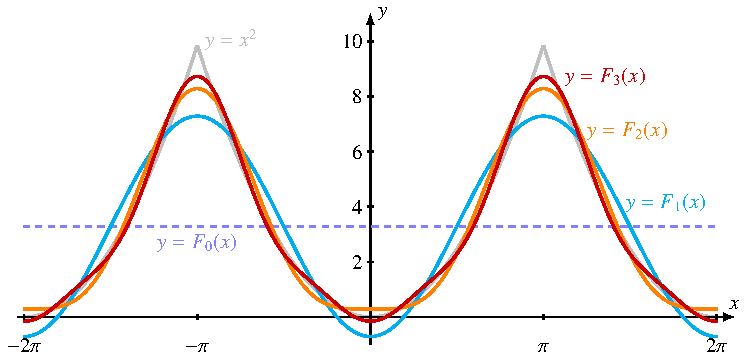
\includegraphics{papers/basel/images/fourier.pdf}
\caption{Periodische Fortsetzung von $f(x) = x^2$ mit den Fourierpolynomen
$F_0$ bis $F_3$.}
\end{figure}


Das nullte Fourier-Polynom dieser Funktion ist nicht besonders, denn es handelt sich
lediglich um eine konstante Funktion.
Anhand der Beobachtung dieser Polynome wird deutlich, dass die Näherung immer
besser wird, wenn man höhere Fourier-Polynome $F_n$ betrachtet.
Dabei ist jedoch zu präzisieren, dass die Aussage \glqq unendlich viele Fourier-Polynome
sind erforderlich\grqq{} nicht ganz korrekt formuliert ist:
Selbst glatte Funktionen $f \in C^\infty([-\pi,\pi])$ besitzen eine Fourier-Reihe
und lassen sich nicht durch ein endliches trigonometrisches Polynom exakt darstellen,
sofern sie nicht selbst bereits von dieser Form sind.
Polynome allein reichen also grundsätzlich nicht aus --- es ist stets die volle
Fourier-Reihe
\[
f(x) = \frac{a_0}{2} + \sum_{k=1}^{\infty} \bigl(a_k \cos(kx) + b_k \sin(kx)\bigr)
\]
erforderlich.
Die Differenzierbarkeit der Funktion beeinflusst dabei die \emph{Konvergenzgeschwindigkeit}:
Je glatter $f$ ist, desto schneller fallen die Fourier-Koeffizienten ab, und
desto weniger Terme werden benötigt, um eine gute Näherung zu erzielen.
Für $f(x) = x^2$ hingegen hat die periodische Fortsetzung an den Randpunkten
$\pm\pi$ einen Sprung in der Ableitung, weshalb die Konvergenz vergleichsweise
langsam ist --- man sieht dies auch daran, dass in den Abbildungen selbst $F_3$
noch spürbar von der Ausgangsfunktion abweicht.
In dieser Hinsicht ist als Grundlage des Beweises das Theorem heranzuziehen,
das besagt, dass es zu punktweiser Konvergenz kommen wird, weil die Funktion
stetig ist.

\subsection{Berechnung der Fourier-Polynome}
\label{basel:subsection:berechnung-fourierpolynome}

%
% pi2.tex
%
% (c) 2026 Prof Dr Andreas Müller
%
\begin{figure}
\centering
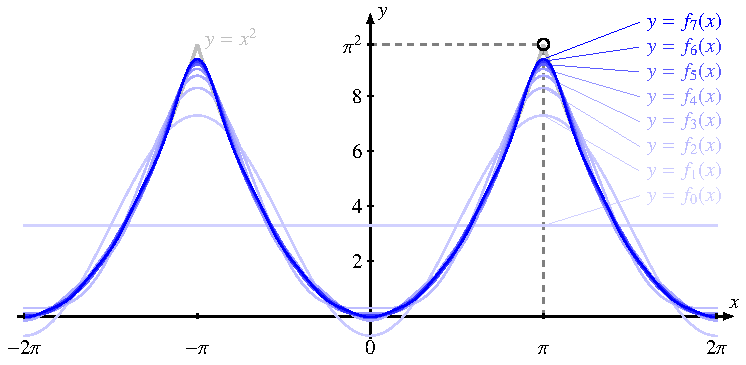
\includegraphics{papers/basel/images/pi2.pdf}
\caption{Im Punkt $\pi$ liegt Konvergenz gegen den Funktionswert $\pi^2$ vor.}
\end{figure}


Ausgangspunkt der Analyse ist die Funktion
\[
f(x) = x^2.
\]
Das allgemeine Fourier-Polynom der Ordnung $n$ ist
\[
F_n f(x)
=
\frac{a_0}{2}
+
\sum_{k=1}^{n}
\bigl(
a_k \cos(kx) + b_k \sin(kx)
\bigr).
\]
Da $f(x) = x^2$ eine gerade Funktion ist, verschwinden alle Sinus-Koeffizienten:
\[
b_k
=
\frac{1}{\pi}
\int_{-\pi}^{\pi} x^2 \sin(kx)\, dx
=
0,
\quad (k > 0).
\]
Der Koeffizient $a_0$ ergibt sich zu
\[
a_0
=
\frac{1}{\pi}
\int_{-\pi}^{\pi} x^2\, dx
=
\frac{x^3}{3\pi}
\bigg|_{-\pi}^{\pi}
=
\frac{2\pi^2}{3}.
\]
Für $k > 0$ liefert partielle Integration
\begin{align*}
a_k
&=
\frac{1}{\pi}
\int_{-\pi}^{\pi} x^2 \cos(kx)\, dx
\\
&=
\frac{1}{k\pi}
\biggl(
x^2 \sin(kx)
\bigg|_{-\pi}^{\pi}
-
2 \int_{-\pi}^{\pi} x \sin(kx)\, dx
\biggr)
\\
&=
-\frac{2}{k\pi}
\int_{-\pi}^{\pi} x \sin(kx)\, dx
\\
&=
\frac{2}{k^2\pi}
\biggl(
x \cos(kx)
\bigg|_{-\pi}^{\pi}
-
\int_{-\pi}^{\pi} \cos(kx)\, dx
\biggr)
\\
&=
\frac{2x}{k^2\pi} \cos(kx)
\bigg|_{-\pi}^{\pi}
=
(-1)^k \frac{4}{k^2},
\quad (k > 0).
\end{align*}
Damit ergibt sich die Fourier-Reihe von $f$:
\[
f(x)
=
\frac{a_0}{2}
+
\sum_{k=1}^{\infty}
\bigl(
a_k \cos(kx) + b_k \sin(kx)
\bigr)
=
\frac{\pi^2}{3}
+
4 \sum_{k=1}^{\infty} \frac{(-1)^k}{k^2} \cos(kx).
\]
Setzt man nun $\pi^2 = f(\pi)$ ein, so erhält man
\begin{align*}
\pi^2
&=
f(\pi)
=
\frac{\pi^2}{3}
+
4 \sum_{k=1}^{\infty} \frac{(-1)^k}{k^2} \cos(k\pi)
=
\frac{\pi^2}{3}
+
\sum_{k=1}^{\infty} \frac{4}{k^2}
\\
\Rightarrow\qquad
\frac{2\pi^2}{3}
&=
4\sum_{k=1}^{\infty} \frac{1}{k^2}
\qquad\Rightarrow\qquad
\sum_{k=1}^{\infty} \frac{1}{k^2}
=
\frac{\pi^2}{6}
%\label{basel:equation:fourier-einsetzen}
\end{align*}
\cite{basel:math.fandom.com}.
